% The 2025 Imsil earthquake swarm: summary report.
% Every number in this file comes from facts.tex (macro \F with a fact key), which notebooks/16_report_figures.ipynb writes from facts.json.
% Compile: tectonic -X compile report.tex
\documentclass[11pt,a4paper]{article}
\usepackage[a4paper,top=2.2cm,bottom=2.4cm,left=2.3cm,right=2.3cm,footskip=1.0cm]{geometry}
\usepackage{fontspec}
\usepackage{unicode-math}
\setmainfont{texgyretermes}[Extension=.otf,UprightFont=*-regular,BoldFont=*-bold,ItalicFont=*-italic,BoldItalicFont=*-bolditalic]
\setsansfont{texgyreheros}[Extension=.otf,UprightFont=*-regular,BoldFont=*-bold,ItalicFont=*-italic,BoldItalicFont=*-bolditalic]
\setmathfont{texgyretermes-math.otf}
\usepackage{microtype}
\usepackage{graphicx}
\usepackage{booktabs}
\usepackage{array}
\usepackage{tabularx}
\usepackage{xcolor}
\usepackage[font=small,labelfont=bf,labelsep=period,skip=5pt,justification=justified]{caption}
\usepackage[authoryear,round]{natbib}
\usepackage[explicit]{titlesec}
\usepackage{enumitem}
\usepackage{placeins}
\usepackage[hidelinks,pdfusetitle]{hyperref}

\definecolor{headblue}{RGB}{28,57,120}
\titleformat{\section}{\sffamily\bfseries\large\color{headblue}}{\thesection}{0.6em}{#1}
\titleformat{\subsection}{\sffamily\bfseries\normalsize}{\thesubsection}{0.6em}{#1}
\titlespacing*{\section}{0pt}{12pt plus 3pt minus 2pt}{5pt plus 1pt}
\titlespacing*{\subsection}{0pt}{8pt plus 2pt minus 2pt}{3pt plus 1pt}
\setlength{\parskip}{0pt}
\setlength{\parindent}{1.2em}
\linespread{1.05}
\setlength{\bibsep}{2pt plus 1pt}
\renewcommand{\bibfont}{\small}
\setlist{itemsep=1pt,topsep=3pt,leftmargin=1.6em}
\renewcommand{\topfraction}{0.95}
\renewcommand{\bottomfraction}{0.8}
\renewcommand{\textfraction}{0.05}
\renewcommand{\floatpagefraction}{0.75}
\setcounter{topnumber}{2}
\setcounter{totalnumber}{3}

% facts.tex -- written by notebooks/16_report_figures.ipynb from facts.json; do not edit by hand.
% generated 2026-10-14T18:24:05+09:00; 228 macros.
\makeatletter
\newcommand\FactDef[2]{\expandafter\def\csname fact@#1\endcsname{#2}}
\DeclareRobustCommand\F[1]{\ifcsname fact@#1\endcsname\csname fact@#1\expandafter\endcsname\else\PackageError{facts}{Undefined fact #1}{Add it to notebook 16}\fi}
\makeatother
\FactDef{a.A1}{14:17:35}
\FactDef{a.A1_ml}{0.3}
\FactDef{a.A1_ntpl}{3}
\FactDef{a.A1_ratio}{0.025}
\FactDef{a.A1_tpl}{400001}
\FactDef{a.A2}{14:17:39}
\FactDef{a.A2_ml}{0.5}
\FactDef{a.A2_ntpl}{7}
\FactDef{a.A2_ratio}{0.043}
\FactDef{a.A2_tpl}{400007}
\FactDef{a.A3}{14:43:15}
\FactDef{a.A3_ml}{0.3}
\FactDef{a.A3_ntpl}{6}
\FactDef{a.A3_ratio}{0.024}
\FactDef{a.A3_tpl}{400007}
\FactDef{a.along}{+35 to +186}
\FactDef{a.bin1}{0.016–0.032}
\FactDef{a.bin2}{0.032–0.050}
\FactDef{a.cc_S_med}{0.43}
\FactDef{a.cc_S_rng}{−0.11–0.92}
\FactDef{a.cc_imsb}{0.80–0.92}
\FactDef{a.cc_low}{0.11}
\FactDef{a.cc_mid}{0.24–0.67}
\FactDef{a.ex95}{83–130}
\FactDef{a.ey95}{20–35}
\FactDef{a.ez95}{36–67}
\FactDef{a.kma_share}{16\% / 43\% / 100\%}
\FactDef{a.n99}{16}
\FactDef{a.nsta_links}{8–9}
\FactDef{a.off_jlsa}{38}
\FactDef{a.off_kch2}{41}
\FactDef{a.off_nawb}{93}
\FactDef{a.robust}{256–328}
\FactDef{a.south}{266–305}
\FactDef{a.sp_joint}{168}
\FactDef{a.sp_res}{24}
\FactDef{a.sp_solo}{38}
\FactDef{a.up}{−86 to −9}
\FactDef{b.imsb_x}{2.0}
\FactDef{b.jasa_share}{0.182}
\FactDef{b.jasa_x}{4.6}
\FactDef{b.kma20}{23}
\FactDef{b.kma20_coinc}{0}
\FactDef{b.sim}{0.39 (0.25–0.76)}
\FactDef{data.fmf_maxd}{59}
\FactDef{data.fmf_s_on_z}{NAWB, KWJ2}
\FactDef{data.long_s_on_z_n}{9}
\FactDef{data.n_days}{151}
\FactDef{data.n_fmf_sta}{22}
\FactDef{data.n_sta}{54}
\FactDef{data.nearest}{IMSB (6.9 km)}
\FactDef{dl.box_after}{55}
\FactDef{dl.box_before}{31}
\FactDef{dl.box_swarm}{39}
\FactDef{dl.days}{153}
\FactDef{dl.kma_imsil}{24 of 24}
\FactDef{dl.kma_region}{86 of 89}
\FactDef{dl.n_A}{529}
\FactDef{dl.n_B}{659}
\FactDef{dl.n_P}{484,833}
\FactDef{dl.n_S}{638,314}
\FactDef{dl.n_box}{125}
\FactDef{dl.n_box_AB}{84}
\FactDef{dl.n_located}{1,695}
\FactDef{dl.shallow_box}{46}
\FactDef{fmf.late}{04:23:32}
\FactDef{fmf.n_10f}{210}
\FactDef{fmf.n_10nf}{235}
\FactDef{fmf.n_12f}{187}
\FactDef{fmf.n_12nf}{194}
\FactDef{fmf.n_det}{235}
\FactDef{fmf.n_new}{207}
\FactDef{fmf.n_ref}{28}
\FactDef{fmf.n_tpl}{28}
\FactDef{fmf.n_window}{234}
\FactDef{fmf.selfcc_aligned}{1.000}
\FactDef{fmf.selfcc_frozen}{0.841}
\FactDef{fmf.top_tpl}{400005}
\FactDef{fmf.top_tpl_eid}{20251102202656}
\FactDef{fmf.top_tpl_n}{51}
\FactDef{geo.dip}{88.2}
\FactDef{geo.hgt}{235}
\FactDef{geo.len}{241}
\FactDef{geo.n99}{15}
\FactDef{geo.rms}{7.4}
\FactDef{geo.strike}{268.7}
\FactDef{jr.dip_ci}{87–90°}
\FactDef{jr.ext}{210, 29, 209}
\FactDef{jr.hw_det}{16.6, 17.1, 75.9}
\FactDef{jr.hw_ref}{1.8, 1.3, 1.2}
\FactDef{jr.n25}{101}
\FactDef{jr.n25_det}{73}
\FactDef{jr.n_rel}{212}
\FactDef{jr.n_rel_det}{184}
\FactDef{jr.strike_ci}{267–271°}
\FactDef{kma.dur}{4.5}
\FactDef{kma.ml}{1.0–1.9}
\FactDef{kma.mlmax_t}{20:38:35}
\FactDef{kma.n}{24}
\FactDef{kma.t0}{20:05}
\FactDef{kma.t0_kst}{05:05}
\FactDef{kma.t1}{00:35}
\FactDef{kma.t1_kst}{09:35}
\FactDef{long.B_first}{September 2023}
\FactDef{long.B_last}{March 2025}
\FactDef{long.imsb_start}{2019-03-18}
\FactDef{long.n}{6,369}
\FactDef{long.nA}{3}
\FactDef{long.nB}{12}
\FactDef{long.nC}{7}
\FactDef{long.n_burst}{6,135}
\FactDef{long.n_days}{3,198}
\FactDef{long.n_other}{22}
\FactDef{long.n_swarm}{212}
\FactDef{long.stack_n}{400}
\FactDef{mag.mw_min}{0.4}
\FactDef{mag.mw_ref}{2.3}
\FactDef{mag.n_above_floor}{95}
\FactDef{mag.n_noise}{140}
\FactDef{meta.date}{14 October 2026}
\FactDef{mig.D05}{0.50}
\FactDef{mig.D05_ci}{0.42–0.74}
\FactDef{mig.D1}{0.59}
\FactDef{mig.D1_ci}{0.42–0.67}
\FactDef{mig.D2}{0.63}
\FactDef{mig.D2_ci}{0.48–0.69}
\FactDef{mig.bf_in}{12 of 65}
\FactDef{mig.bf_t0}{24.3}
\FactDef{mig.bf_t0_ci}{1.0–25.9}
\FactDef{ml.anchors}{0}
\FactDef{ml.dkma_med}{−0.13}
\FactDef{ml.dkma_rms}{0.17}
\FactDef{ml.eurb}{−0.46}
\FactDef{ml.kwj2}{−0.55}
\FactDef{ml.kwj2_B}{+0.15}
\FactDef{ml.n_primary_B}{14}
\FactDef{ml.n_primary_ref}{8 of 28}
\FactDef{ml.nawb}{+0.54}
\FactDef{ml.nawb_B}{+0.04}
\FactDef{p.bound}{25}
\FactDef{p.box_lat}{34.85–36.25° N}
\FactDef{p.box_lon}{126.50–128.10° E}
\FactDef{p.err}{5}
\FactDef{p.fmf_band}{5–20}
\FactDef{p.fmf_mad}{10}
\FactDef{p.fmf_merge}{4}
\FactDef{p.fmf_minsta}{4}
\FactDef{p.fmf_pre}{0.5}
\FactDef{p.fmf_pwin}{1.5}
\FactDef{p.fmf_snr}{1.2}
\FactDef{p.fmf_swin}{2.0}
\FactDef{p.fs}{100}
\FactDef{p.gap}{180}
\FactDef{p.haenam_floor}{0.20}
\FactDef{p.haenam_mad}{12}
\FactDef{p.n_p}{3}
\FactDef{p.n_picks}{6}
\FactDef{p.n_ps}{2}
\FactDef{p.n_s}{3}
\FactDef{p.nboot}{1,000}
\FactDef{p.num}{7}
\FactDef{p.obscc}{4}
\FactDef{p.pmin}{0.2}
\FactDef{p.rms}{1}
\FactDef{p.xc_band}{5–20}
\FactDef{p.xc_cc}{0.7}
\FactDef{p.xc_interp}{1,000}
\FactDef{p.xc_win}{0.5}
\FactDef{p.zfloor}{10}
\FactDef{p.zlim}{0–30}
\FactDef{pk.D_ours}{0.34–0.40}
\FactDef{pk.D_theirs}{0.45–0.61}
\FactDef{pk.b_c2}{1.53–1.02}
\FactDef{pk.b_ours}{1.33 ± 0.18}
\FactDef{pk.b_theirs}{1.40 ± 0.07}
\FactDef{pk.band_theirs}{10–40}
\FactDef{pk.below}{71–95\%}
\FactDef{pk.below_mw}{0.8}
\FactDef{pk.dd_sep}{520}
\FactDef{pk.depth_dd}{12.8–13.0}
\FactDef{pk.depth_hyp}{13.79}
\FactDef{pk.depth_theirs}{13.6–14.0}
\FactDef{pk.epi_kim1983}{N −128 m, E −148 m}
\FactDef{pk.ext}{237 × 225}
\FactDef{pk.ext_theirs}{300 × 350}
\FactDef{pk.extra}{263}
\FactDef{pk.mag_rms}{0.11}
\FactDef{pk.n_theirs}{498}
\FactDef{pk.plane_theirs}{89° / 89°}
\FactDef{pk.share}{47\%}
\FactDef{pk.share_P1}{47\%}
\FactDef{pk.share_P2}{44\%}
\FactDef{pk.share_P3}{55\%}
\FactDef{pk.share_P4}{64\%}
\FactDef{pk.spear}{0.59}
\FactDef{pk.spear_p}{0.004}
\FactDef{pk.sta_theirs}{60}
\FactDef{pk.t_dist}{−14 / −22}
\FactDef{pk.t_time}{−2.1 / +2.8}
\FactDef{pk.thick}{37}
\FactDef{prev.n_ev}{18}
\FactDef{prev.n_sta}{11}
\FactDef{rel.d6}{6.2}
\FactDef{rel.dip04}{84–95°}
\FactDef{rel.ext04}{126 m east–west, 27 m north–south and 186 m in depth}
\FactDef{rel.flip04}{134}
\FactDef{rel.kma_in_ref}{22 of 24}
\FactDef{rel.med95_E}{1.9}
\FactDef{rel.med95_N}{1.3}
\FactDef{rel.med95_Z}{2.1}
\FactDef{rel.n_ref}{28}
\FactDef{rel.n_sub}{34}
\FactDef{rel.plane04}{272° / 87°}
\FactDef{rel.prev_n}{17}
\FactDef{rel.prev_res}{1, 1, 2}
\FactDef{rel.strike04}{268–284°}
\FactDef{smoke.dP}{0.01}
\FactDef{smoke.dS}{0.032}
\FactDef{smoke.depth_km}{14.6}
\FactDef{smoke.epi_km}{0.11}
\FactDef{t.box_swarm}{40}
\FactDef{t.first}{19:57:38}
\FactDef{t.last_window}{00:53:41}
\FactDef{t.span_h}{5}
\FactDef{vet.ab_iso}{58}
\FactDef{vet.ab_near}{18}
\FactDef{vet.iso}{114}
\FactDef{vet.near}{93}


\newcommand{\Mw}{\ensuremath{M_\mathrm{w}}}
\newcommand{\ML}{\ensuremath{M_\mathrm{L}}}
\newcommand{\msq}{m\textsuperscript{2}/s}
\newcommand{\figref}[1]{Figure~\ref{#1}}

\hypersetup{pdftitle={The 2025 Imsil earthquake swarm},pdfauthor={Min-Seong Seo}}

\begin{document}

\begin{center}
{\sffamily\bfseries\LARGE\color{headblue} The 2025 Imsil earthquake swarm,\\[2pt] southwestern Korea\par}
\vspace{4pt}
{\sffamily\large Detection, relocation, template matching and earlier activity on the source fault\par}
\vspace{8pt}
{\normalsize Min-Seong Seo\par}
{\small School of Earth and Environmental Sciences, Seoul National University\par}
\vspace{2pt}
{\small Summary report, \F{meta.date}\par}
\end{center}

\vspace{2pt}
\noindent\begin{minipage}{\textwidth}
\small
\textbf{\sffamily Abstract.}
On 2 November 2025 (UTC), a swarm of small earthquakes occurred at mid-crustal depth beneath Imsil, southwestern Korea. The Korea Meteorological Administration (KMA) listed \F{kma.n} events of local magnitude \ML\ \F{kma.ml} within \F{kma.dur}~h.
We rebuilt the catalog with the detection, relocation and template-matching pipeline adopted for the Haenam sequences, changing only the region values. Every change of setting was compared before adoption and recorded.
Template matching with the \F{fmf.n_tpl} best-located events finds \F{fmf.n_det} events, \F{fmf.n_new} of them new. All but one fall within \F{t.span_h}~h on 2--3 November, and the one exception follows at \F{fmf.late} on 3 November.
The \F{jr.n25} events whose 95\,\% location half-widths are at most \F{p.bound}~m outline a near-vertical plane striking \F{geo.strike}° and dipping \F{geo.dip}°. Their root-mean-square (RMS) distance from the plane is \F{geo.rms}~m, and they span about \F{geo.len}~m along strike and \F{geo.hgt}~m in depth.
The swarm started low in the west and spread east and up the plane. A diffusion front fitted to the outermost events gives a hydraulic diffusivity of \F{mig.D05}--\F{mig.D2}~\msq, depending on the length of the fit window.
A template-matching scan of \F{long.n_days} days from 2018 to 2026 finds three earlier events on 15 April 2019. Their amplitudes are \F{a.A3_ratio}--\F{a.A2_ratio} times that of the \ML\ 1.9 event, and KMA did not catalog them.
Relocated together with the 2025 swarm, they lie \F{a.south}~m south of the 2025 plane, at the same depths and within its along-strike extent. They therefore point to a second, parallel fault strand that was active six years before the swarm.
Compared with \citet{Park2026}, who studied the same swarm, our catalog holds \F{pk.share} of their events. The difference is in events below their \Mw\ \F{pk.below_mw}, and it follows from their larger network, wider frequency band and lower detection threshold.
\end{minipage}
\vspace{4pt}

\section{The swarm and the data}

The swarm occurred on 2--3 November 2025 between \F{kma.t0} and \F{kma.t1} UTC (\F{kma.t0_kst}--\F{kma.t1_kst} Korean time on 3 November). Its largest event was the \ML\ 1.9 at \F{kma.mlmax_t} UTC. Before this study, the swarm had been analyzed only with an earlier, quicker pipeline: hand picks on the \ML\ 1.9, deep-learning detection at \F{prev.n_sta} stations over three days, and a double-difference relocation of \F{prev.n_ev} events.

We used the continuous records of the \F{data.n_sta} KMA stations (network code KS) within 100~km of the swarm (\figref{fig:map}), from 1 September 2025 to 31 January 2026 (\F{dl.days} days). No data of the Korea Institute of Geoscience and Mineral Resources (KIGAM) exist for 2025, and the nearest Chonnam National University stations started in September 2026, so the network is KS only. The nearest station is \F{data.nearest}. Template matching used the \F{data.n_fmf_sta} stations within \F{data.fmf_maxd}~km.

\begin{figure}[t]
\centering
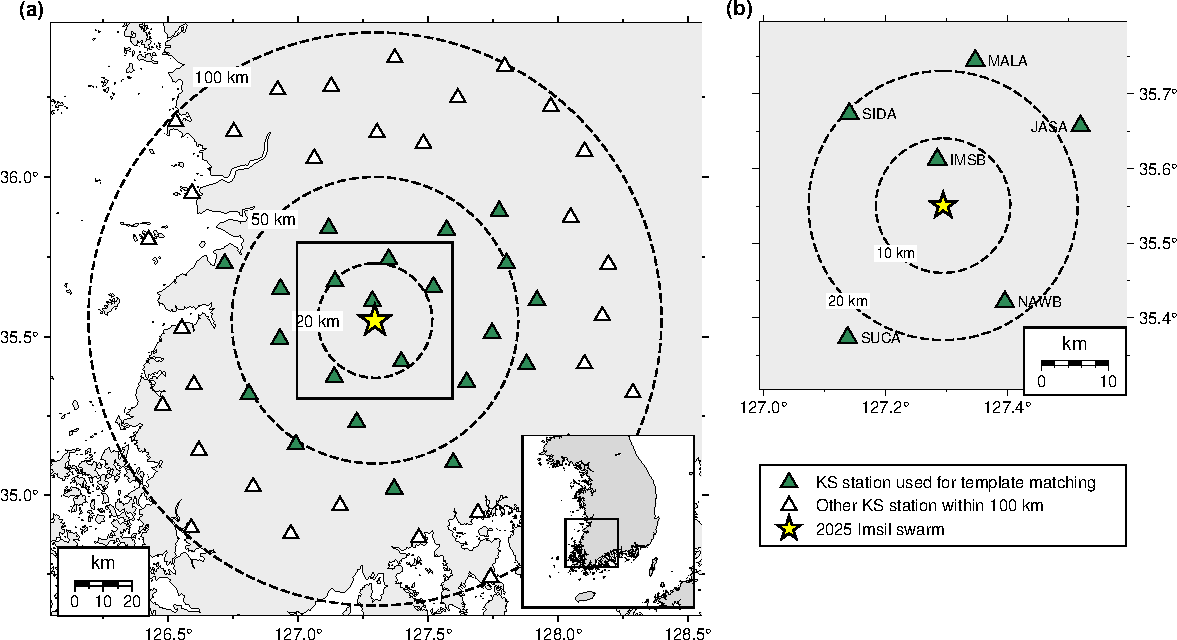
\includegraphics[width=\textwidth]{figures/Figure_01_station_map.pdf}
\caption{Stations. (a) The \F{data.n_sta} KS stations within 100~km of the swarm (star), with the \F{data.n_fmf_sta} stations used for template matching in green; dashed circles at 20, 50 and 100~km. Inset: location in Korea. (b) The stations within the box of panel (a), with names.}
\label{fig:map}
\end{figure}

\section{Methods}

The pipeline is the one adopted for the 2020--2026 Haenam sequences and the 2024 Buan sequence \citep{Seo2025}. Its code was copied unchanged: the picking, association, location, waveform export, magnitude and template-matching scan modules are byte-identical to the Haenam code, as checked by checksum. Only the region values (association box, relocation box, station table, period) were changed, each by a stated rule. Each choice that the Haenam rules did not settle was given evidence in a numbered notebook and recorded in a decision log (Section~\ref{sec:open}). Table~\ref{tab:pipeline} lists the settings.

\textbf{Detection and location.} A deep-learning phase picker of the PhaseNet family \citep{Zhu2019} was applied at \F{p.fs} samples per second, keeping picks with probability $\ge$\,\F{p.pmin}. Picks were grouped into events (\emph{association}) with PyOcto \citep{Munchmeyer2024} within \F{p.box_lat}, \F{p.box_lon} and \F{p.zlim}~km depth. An event required at least \F{p.n_picks} picks, among them \F{p.n_p} P and \F{p.n_s} S picks, and \F{p.n_ps} stations with both. Events were located with HYPOINVERSE \citep{Klein2002} in the layered model of \citet{KimKim1983}. On the swarm days, the picker found all \F{kma.n} KMA events. The \ML\ 1.9 located \F{smoke.epi_km}~km from its hand-pick epicenter at \F{smoke.depth_km}~km depth. The median differences between automatic and hand picks were \F{smoke.dP}~s for P and \F{smoke.dS}~s for S.

\textbf{Relocation.} Events in the Imsil box that passed a location-quality gate were relocated by the double-difference method \citep{Waldhauser2000}, which solves for the relative positions of nearby events. The gate required an azimuthal gap below \F{p.gap}°, more than \F{p.num} phases, an RMS residual below \F{p.rms}~s, errors below \F{p.err}~km and a depth of at least \F{p.zfloor}~km. Differential times came from the picks and from waveform cross-correlation: \F{p.xc_band}~Hz, windows of $\pm$\F{p.xc_win}~s, interpolation to \F{p.xc_interp}~Hz, correlation coefficient (CC) $\ge$\,\F{p.xc_cc}, and at least \F{p.obscc} observations per event pair. Uncertainties are the 2.5--97.5\,\% ranges of \F{p.nboot} bootstrap replicas, each with the data resampled. The \emph{reference catalog} keeps the events whose 95\,\% half-widths are at most \F{p.bound}~m in east, north and depth separately. Planes were fitted by singular-value decomposition (SVD), a total-least-squares fit to the hypocenters.

\textbf{Magnitudes.} Local magnitudes come from the scale of \citet{Sheen2018}, computed as in Haenam. For relative size we also use the ratio of 5--20~Hz S-wave peak displacement to that of the \ML\ 1.9 event, recorded on the same channel so that the instrument response cancels. Each event's ratio is the median over the channels on which the \ML\ 1.9 has a signal-to-noise ratio of at least 300. The scale of \citet{Park2026} converts this ratio to their \Mw.

\textbf{Template matching.} The \F{fmf.n_tpl} events of the reference catalog served as templates for a network matched filter \citep{Beauce2018}. The filter used \F{p.fmf_band}~Hz, a \F{p.fmf_pwin}~s P window on the vertical and \F{p.fmf_swin}~s S windows, each starting \F{p.fmf_pre}~s before the pick, at \F{data.n_fmf_sta} stations; S was taken on the vertical at \F{data.fmf_s_on_z}, whose horizontals were re-instrumented during the period. A detection must exceed \F{p.fmf_mad} times the median absolute deviation (MAD) of the network correlation, computed per day and per station configuration, with at least \F{p.fmf_minsta} stations; hits closer than \F{p.fmf_merge}~s are merged. Two settings differ from Haenam. First, every day trace is shifted onto the exact 10~ms sample grid before templates are cut. Without this shift, templates at stations sampling off the grid were compared with the wrong sample, and their self-detection CC was \F{fmf.selfcc_frozen} instead of \F{fmf.selfcc_aligned}. Second, the threshold is \F{p.fmf_mad}~$\times$~MAD with no absolute CC floor, instead of Haenam's \F{p.haenam_mad}~$\times$~MAD with a CC floor of \F{p.haenam_floor}. The catalog sizes for the four combinations were \F{fmf.n_12f}, \F{fmf.n_12nf}, \F{fmf.n_10f} and \F{fmf.n_10nf}.

\textbf{Joint relocation of detections.} Each new detection inherits its template's picks, shifted to the detection origin; the picks only place the correlation windows. Detections are tied to the \F{fmf.n_tpl} reference events and to each other by cross-correlation times alone, with the relocation settings above, the bootstrap and the 25~m rule.

\textbf{Long scan.} The same templates were run over every day from 1 January 2018 to 3 October 2026, \F{long.n_days} days. The vertical was used for S at the \F{data.long_s_on_z_n} stations whose response changed during these years. KS.IMSB, the nearest station, has records from \F{long.imsb_start}.

\begin{table}[t]
\centering
\small
\caption{Pipeline and settings. The detection and relocation settings equal Haenam's; the two template-matching changes are explained in the text.}
\label{tab:pipeline}
\begin{tabularx}{\textwidth}{@{}l>{\raggedright\arraybackslash}X@{}}
\toprule
Step & Settings \\
\midrule
Stations and period & \F{data.n_sta} KS stations within 100~km; 1 Sep 2025 -- 31 Jan 2026 (\F{dl.days} days) \\
Picking & PhaseNet family, \F{p.fs}~Hz, probability $\ge$\,\F{p.pmin} \\
Association & PyOcto; $\ge$\,\F{p.n_picks} picks, $\ge$\,\F{p.n_p} P, $\ge$\,\F{p.n_s} S, \F{p.n_ps} stations with both \\
Location & HYPOINVERSE, Kim \& Kim (1983) model \\
Relocation & double difference; picks + cross-correlation (\F{p.xc_band}~Hz, CC $\ge$\,\F{p.xc_cc}); \F{p.nboot} bootstrap replicas; reference = 95\,\% half-widths $\le$\,\F{p.bound}~m \\
Local magnitude & \citet{Sheen2018} scale, Haenam implementation \\
Template matching & \F{fmf.n_tpl} templates, \F{data.n_fmf_sta} stations, \F{p.fmf_band}~Hz; P \F{p.fmf_pwin}~s, S \F{p.fmf_swin}~s; \F{p.fmf_mad}~$\times$~MAD, no CC floor, $\ge$\,\F{p.fmf_minsta} stations; grid-aligned traces \\
Long scan & same templates, 2018-01-01 to 2026-10-03 (\F{long.n_days} days) \\
\bottomrule
\end{tabularx}
\end{table}

\section{Results}

\subsection{Deep-learning catalog and the reference events}

The detection run located \F{dl.n_located} events in and around the region from \F{dl.n_P} P and \F{dl.n_S} S picks. It recovered \F{dl.kma_imsil} KMA-listed Imsil events and \F{dl.kma_region} KMA events in the association box. The Imsil box holds \F{dl.n_box} events: \F{dl.box_before} before the swarm, \F{dl.box_swarm} during it and \F{dl.box_after} after it. Apart from the swarm, the box contains mainly shallow daytime events, probably quarry blasts, which the depth floor removes (\F{dl.shallow_box} of the well-located ones).

Of the \F{rel.n_sub} relocated events, \F{rel.n_ref} meet the 25~m rule, \F{rel.kma_in_ref} KMA-listed events among them. Their median 95\,\% half-widths are \F{rel.med95_E}, \F{rel.med95_N} and \F{rel.med95_Z}~m in east, north and depth. They occupy \F{rel.ext04}, on a plane of \F{rel.plane04} (strike/dip). The earlier relocation of \F{prev.n_ev} events agrees after one rigid shift of the whole cluster: the median residuals of the \F{rel.prev_n} matched events are \F{rel.prev_res}~m in east, north and depth.

\subsection{Magnitudes}

Only \F{ml.n_primary_ref} reference events have a local magnitude from at least three stations with a pick and a signal-to-noise ratio of at least 2. Most swarm events are too small for the KS network at its usual distances. Where both exist, our \ML\ minus the KMA \ML\ has a median of \F{ml.dkma_med} and an RMS of \F{ml.dkma_rms}. Three stations have large residuals: NAWB \F{ml.nawb}, KWJ2 \F{ml.kwj2} and EURB \F{ml.eurb}. These stations carry response epochs that differ between the two metadata sources. With the KMA response files instead of the master metadata, the NAWB and KWJ2 residuals become \F{ml.nawb_B} and \F{ml.kwj2_B}, and \F{ml.n_primary_B} events get a magnitude. Which source to use is still open (D4). The Haenam relative-magnitude method needs anchor events with at least 20 picked stations; Imsil has \F{ml.anchors}, so that method does not transfer. For this reason the timeline uses amplitude ratios (\figref{fig:time}a).

\subsection{Template matching}

Template matching finds \F{fmf.n_det} events: the \F{fmf.n_ref} templates and \F{fmf.n_new} new detections (\figref{fig:time}). \F{fmf.n_window} fall between \F{t.first} and \F{t.last_window} UTC, and the last follows alone at \F{fmf.late} on 3 November. No other event in the five-month period matches the templates. Template \F{fmf.top_tpl} (event \F{fmf.top_tpl_eid}), a small event that KMA did not list, accounts for the most detections (\F{fmf.top_tpl_n}). Of the new detections, \F{vet.iso} are isolated and \F{vet.near} lie within 15~s of a stronger detection. A template could also match the later phases of a larger event at a fixed lag, but the observed lags show no excess over a randomized control. All detections therefore went to relocation, where the correlation links and the bootstrap act as an independent check.

The detections follow the four phases P1--P4 defined by \citet{Park2026} (\figref{fig:time}a). For \F{mag.n_noise} detections the amplitude ratio is within a factor of 2 of the same measurement on the noise before P, so their sizes are upper bounds. In the swarm window, the deep-learning catalog has \F{t.box_swarm} events in the Imsil box and KMA lists \F{kma.n} (\figref{fig:time}b).

\begin{figure}[t]
\centering
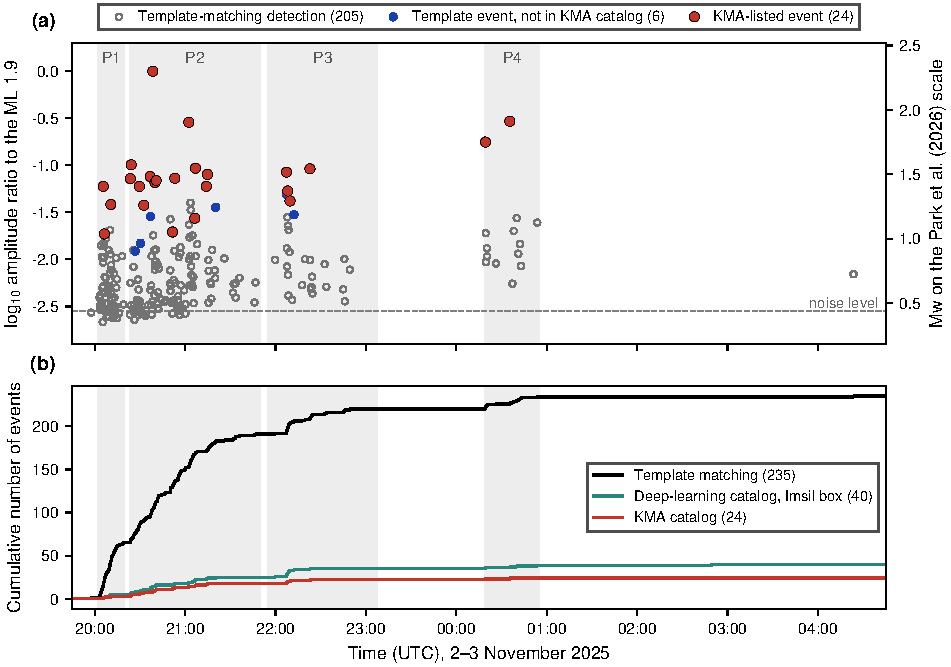
\includegraphics[width=\textwidth]{figures/Figure_02_swarm_timeline.pdf}
\caption{The swarm in time. (a) Size of the \F{fmf.n_det} template-matching events: the 5--20~Hz S-wave peak-displacement ratio to the \ML\ 1.9 (median over the channels on which the \ML\ 1.9 has a signal-to-noise ratio of at least 300). The right axis converts the ratio to \Mw\ with the scale of \citet{Park2026}. Red: KMA-listed; blue: templates not listed by KMA; open: new detections. The dashed line is the median reading of the same measurement before the P arrival (noise). Gray bands: phases P1--P4 of \citet{Park2026}. (b) Cumulative numbers of events: template matching, the deep-learning catalog (Imsil box, 19:30--05:00 UTC) and KMA.}
\label{fig:time}
\end{figure}

\subsection{Geometry}

Of the \F{fmf.n_det} events, \F{jr.n_rel} were relocated (\F{jr.n_rel_det} detections), and \F{jr.n25} meet the 25~m rule: the \F{fmf.n_tpl} templates and \F{jr.n25_det} detections (\figref{fig:geom}). Their median 95\,\% half-widths are \F{jr.hw_ref}~m (templates) and \F{jr.hw_det}~m (detections) in east, north and depth. The SVD plane strikes \F{geo.strike}° and dips \F{geo.dip}° to the north (95\,\% ranges \F{jr.strike_ci} and \F{jr.dip_ci}). The RMS distance from the plane is \F{geo.rms}~m, and 99\,\% of the events lie within \F{geo.n99}~m of it. The events span \F{jr.ext}~m in east, north and depth (95\,\%). Absolute depths of a double-difference cluster are not resolved, because the cluster keeps the mean starting depth of its events. Two relocation runs agree to a few meters in relative position but differ by \F{pk.dd_sep}~m in absolute position. The absolute depth is best taken from the well-recorded single-event locations: \F{pk.depth_hyp}~km.

\begin{figure}[t]
\centering
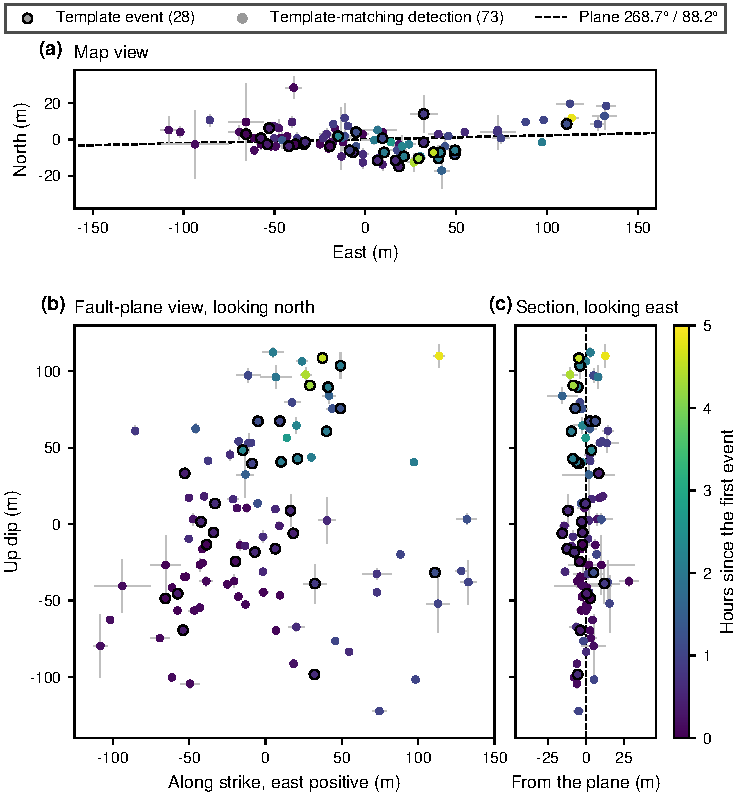
\includegraphics[width=0.86\textwidth]{figures/Figure_03_geometry.pdf}
\caption{Geometry of the \F{jr.n25} events that meet the 25~m rule, colored by time; templates have black edges. Gray bars are 95\,\% half-widths. (a) Map view with the trace of the fitted plane. (b) The plane seen from the south (along strike against up dip). (c) Section along the plane: distance from the plane against up dip. Positions are relative to the centroid.}
\label{fig:geom}
\end{figure}

\subsection{Migration}

The first event, at \F{t.first}, lies at the lower western end of the patch, and later events spread east and up (\figref{fig:geom}b, \figref{fig:mig}b). If a pressure front spreading from the first event triggered the swarm, the outermost events should follow $r^2 = 4\pi D t$, where $D$ is the hydraulic diffusivity \citep{Shapiro1997}. Fits through the front-setting events give $D=$ \F{mig.D05}, \F{mig.D1} and \F{mig.D2}~\msq\ for fit windows of 0.5, 1 and 2~h. Their bootstrap 95\,\% ranges are \F{mig.D05_ci}, \F{mig.D1_ci} and \F{mig.D2_ci}~\msq\ (\figref{fig:mig}a). We also fitted a back front, the inner edge of a quiet zone that opens after the pressure source stops \citep{Parotidis2004}. It is not stable: its start time ranges over \F{mig.bf_t0_ci}~min in resamples, so it is not interpreted. The choice of time scale is still open (D24).

\begin{figure}[t]
\centering
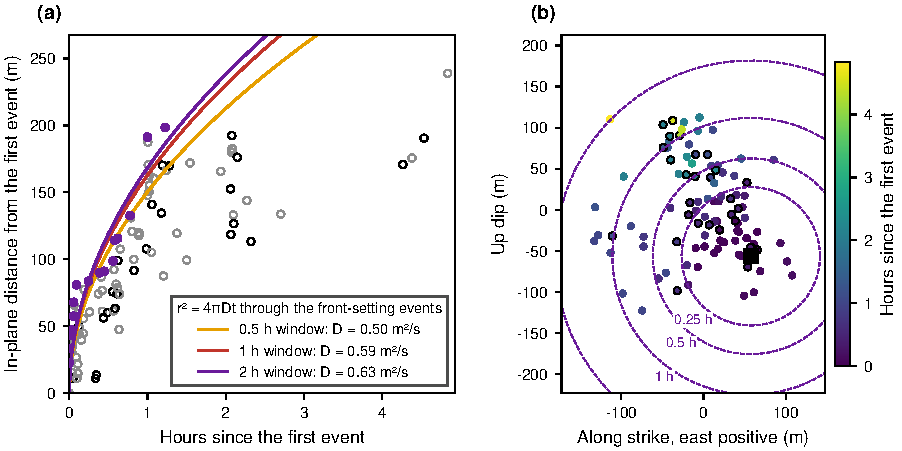
\includegraphics[width=\textwidth]{figures/Figure_04_migration.pdf}
\caption{Migration. (a) In-plane distance from the first event against time; filled symbols are the front-setting events of each fit window, and the curves are $r^2=4\pi Dt$ fits for windows of 0.5, 1 and 2~h. Black-edged: templates. (b) The events on the plane, colored by time; the square is the first event, and the dashed circles are the 2-h front at 0.25, 0.5, 1 and 2~h.}
\label{fig:mig}
\end{figure}

\subsection{Comparison with Park et al. (2026)}

\citet{Park2026} studied the same swarm with one template (the \ML\ 1.9), \F{pk.sta_theirs} stations, a \F{pk.band_theirs}~Hz band and visual vetting. Their per-event catalog is not public, so their side of each comparison is the number printed in their paper (Table~\ref{tab:park}). We reproduce their magnitude scale to \F{pk.mag_rms} RMS on the events whose magnitudes or amplitude ratios they quote. Of the \F{pk.extra} events they have and we lack, \F{pk.below} are below their \Mw\ \F{pk.below_mw}. Their mechanism of the \ML\ 1.9 predicts the ranking of our station P/S amplitude ratios (Spearman correlation \F{pk.spear}, $p=$\,\F{pk.spear_p}). IMSB lies near a P-wave node, which is why its P is weak. They read the fall of waveform similarity during the swarm as a change of the source with time. In our data, the fall is carried by the distance between events ($t=$\,\F{pk.t_dist} at MALA and NAWB) rather than by time ($t=$\,\F{pk.t_time}), that is, by the migration. Their b-value of \F{pk.b_theirs} rests on a magnitude scale with slope 0.73 borrowed from another region. On their scale our b-value is \F{pk.b_ours}, and the same data give \F{pk.b_c2} for slopes from 2/3 to 1. A ``high b-value'' is therefore partly a statement about the borrowed slope.

\begin{table}[t]
\centering
\small
\caption{This study and \citet{Park2026}.}
\label{tab:park}
\begin{tabularx}{\textwidth}{@{}l>{\raggedright\arraybackslash}X>{\raggedright\arraybackslash}X@{}}
\toprule
Topic & \citet{Park2026} & This study \\
\midrule
Catalog & \F{pk.n_theirs} events; \F{pk.sta_theirs} stations; \F{pk.band_theirs}~Hz & \F{fmf.n_det} events (\F{pk.share}); \F{data.n_fmf_sta} stations; \F{p.fmf_band}~Hz \\
Share per phase & -- & P1 \F{pk.share_P1}, P2 \F{pk.share_P2}, P3 \F{pk.share_P3}, P4 \F{pk.share_P4} \\
Depth & \F{pk.depth_theirs}~km & \F{pk.depth_hyp}~km (single-event locations) \\
Plane & \F{pk.plane_theirs} & \F{geo.strike}° / \F{geo.dip}° \\
Extent, along strike $\times$ depth & \F{pk.ext_theirs}~m & \F{pk.ext}~m; \F{pk.thick}~m thick (99\,\%) \\
Diffusivity, their method & \F{pk.D_theirs}~\msq & \F{pk.D_ours}~\msq \\
b-value & \F{pk.b_theirs} & \F{pk.b_ours} on their scale \\
\bottomrule
\end{tabularx}
\end{table}

\subsection{The long scan, 2018--2026}

The long scan returned \F{long.n} detections (\figref{fig:long}):
\begin{itemize}
\item \F{long.n_swarm} in the 2025 swarm window, the control, which reproduces the swarm with the changed S components;
\item \F{long.n_burst} on 6--8 March 2018, which are noise triggers: a median stack of the \F{long.stack_n} strongest shows no arrivals at any station;
\item \F{long.n_other} others, in three groups.
\end{itemize}
The \F{long.nB} detections of group B come from template \F{fmf.top_tpl} alone, between \F{long.B_first} and \F{long.B_last}. Their signal is seen only at JASA, where the stacked envelope rises to \F{b.jasa_x} times the pre-event level (\F{b.imsb_x} at IMSB). Their similarity to each other is low (\F{b.sim}). JASA carries \F{b.jasa_share} of this template's weight, more than for any other template. Group B is therefore a repeating local source near JASA, not activity on the Imsil fault. KMA lists \F{b.kma20} events within 20~km of JASA in 2023--2025, and none of them coincides with a group-B detection. The \F{long.nC} single-template detections of group C show no arrivals. Group A consists of three events on 15 April 2019, each detected by several templates.

\begin{figure}[t]
\centering
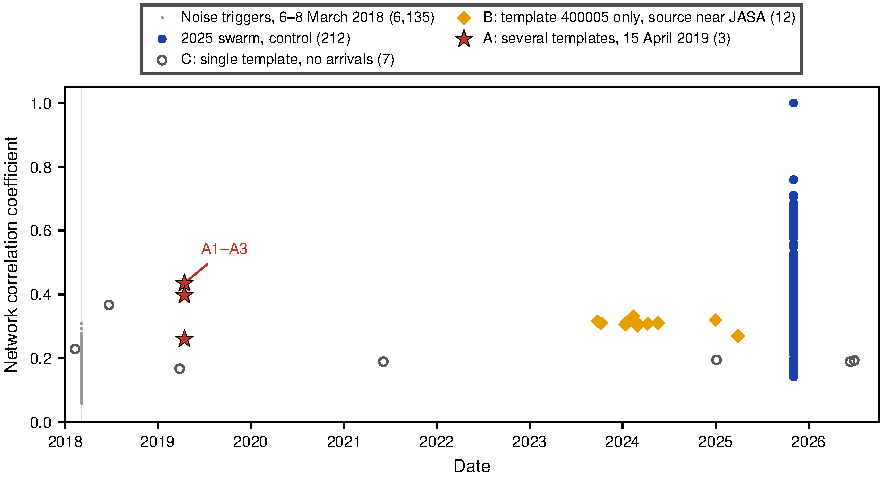
\includegraphics[width=\textwidth]{figures/Figure_05_long_scan.pdf}
\caption{Template-matching detections from 1 January 2018 to 3 October 2026 (\F{long.n_days} days), by network correlation coefficient. Gray band and dots: the noise burst of 6--8 March 2018.}
\label{fig:long}
\end{figure}

\subsection{The events of 15 April 2019}

A1 (\F{a.A1}~UTC), A2 (\F{a.A2}) and A3 (\F{a.A3}) were detected by \F{a.A1_ntpl}, \F{a.A2_ntpl} and \F{a.A3_ntpl} templates. Their waveforms repeat those of the 2025 templates (\figref{fig:wave}). The correlation in the S window is \F{a.cc_imsb} at the nearest station, IMSB, and \F{a.cc_mid} at JEU2, GKSA and MALA. It is at most \F{a.cc_low} at SUCA and JLSA, where S is taken on the vertical and the stations were re-instrumented between 2019 and 2025. Their S amplitudes are \F{a.A1_ratio}, \F{a.A2_ratio} and \F{a.A3_ratio} times that of the \ML\ 1.9, about \ML\ \F{a.A1_ml}--\F{a.A2_ml} if \ML\ scales one-to-one with log amplitude. Of the 2025 swarm events with amplitude ratios of \F{a.bin1}, \F{a.bin2} and larger, KMA cataloged \F{a.kma_share}, so events of this size are usually missing from its catalog.

Relocated together with all 2025 events and with the same settings, A1--A3 lie \F{a.south}~m south of the 2025 plane (\figref{fig:loc}). For comparison, 99\,\% of the 25~m events of the same run lie within \F{a.n99}~m of the plane. Their 95\,\% half-widths are \F{a.ey95}~m north--south, \F{a.ex95}~m east--west and \F{a.ez95}~m in depth. In the plane they lie \F{a.along}~m along strike and \F{a.up}~m up dip from the swarm centroid, inside the swarm's extent and at its depths (\figref{fig:loc}c). Their correlation links come from \F{a.nsta_links} stations, because detections inherit the picks of their templates. At some stations the 2019-to-2025 links carry median residuals that point to timing or instrument changes: NAWB +\F{a.off_nawb}~ms, KCH2 $-$\F{a.off_kch2}~ms and JLSA $-$\F{a.off_jlsa}~ms. Solved again against the fixed swarm without these stations, or with stable-epoch stations only, the events stay \F{a.robust}~m south.

Relocated alone, the three events cannot move as a group. Every equation compares one of them with another, so their centroid stays at its starting position, the location of their templates. The solo run therefore cannot test the offset. It does show how they lie relative to each other: within \F{a.sp_solo}~m alone and \F{a.sp_res}~m in the re-solve, against \F{a.sp_joint}~m in the joint run, whose along-strike spread is within its uncertainty (\figref{fig:loc}d). A1--A3 are best read as a tight group \F{a.south}~m south of the 2025 plane, on a structure parallel to it.

\begin{figure}[t]
\centering
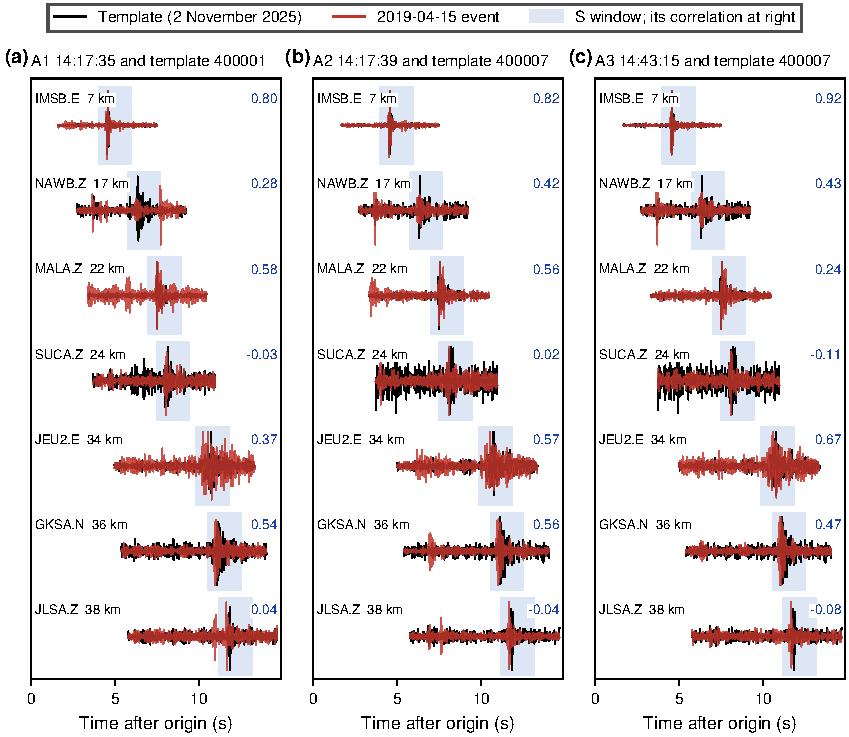
\includegraphics[width=\textwidth]{figures/Figure_06_2019_waveforms.pdf}
\caption{Waveforms of A1--A3 (red) against their templates (black) at the seven nearest stations with a template S pick, 5--20~Hz, each trace normalized. The S window (shaded) is the one the scan correlates; the number is its correlation at the detection time. S is shown on the horizontal component with the higher correlation, or on the vertical where the scan uses the vertical.}
\label{fig:wave}
\end{figure}

\begin{figure}[t]
\centering
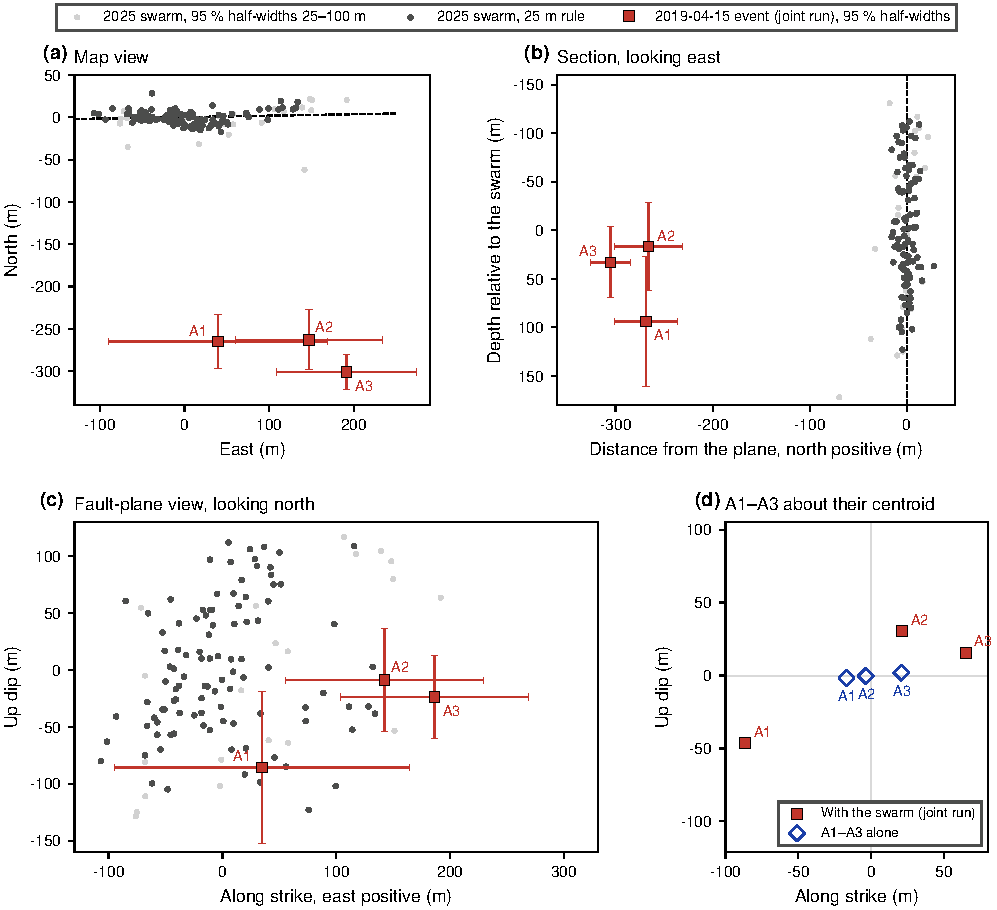
\includegraphics[width=\textwidth]{figures/Figure_07_2019_location.pdf}
\caption{Position of A1--A3 relative to the 2025 swarm (joint relocation; error bars are 95\,\% half-widths). (a) Map view with the trace of the 2025 plane. (b) Section looking east: distance from the plane against depth relative to the swarm centroid. (c) Fault-plane view. (d) A1--A3 about their own centroid in the joint run and in the relocation of the three events alone.}
\label{fig:loc}
\end{figure}

\FloatBarrier
\section{Interpretation}

The swarm activated a near-vertical patch about \F{geo.len}~m long on an east--west plane, starting at its lower western end and spreading up and east. The spreading follows a diffusion front with $D=$ \F{mig.D05}--\F{mig.D2}~\msq, consistent with a pressure front. The events of 15 April 2019 show that the source region was active six years earlier, on a structure \F{a.south}~m south of the 2025 plane and parallel to it. The three events are small and not cataloged by KMA. The joint relocation, the robustness tests and the waveform similarity all support this reading. Two limits remain. The 2019 events are tied to the swarm at only \F{a.nsta_links} stations. Some of those stations changed timing or instruments between 2019 and 2025, although removing them does not change the result. An independent check, with picks of the 2019 events themselves or with S$-$P times that do not depend on station clocks, has not yet been made. No other detection between 2018 and 2026 is an event on the Imsil source.

\section{Open decisions and limitations}
\label{sec:open}

The following settings are still open in the decision log (\texttt{docs/decisions.csv}); each has its evidence in the notebook named.
\begin{itemize}
\item \textbf{D4, response metadata for \ML} (notebooks 05, 05a): the master metadata or the KMA response files; the station residuals at NAWB, KWJ2 and EURB decide.
\item \textbf{D18, magnitude validator}: the Haenam validator quarantines every KMA response file because of a cosmetic warning; it changes the number of magnitudes.
\item \textbf{D5, depth floor of \F{p.zfloor}~km} and \textbf{D6, onset windows} (notebook 04): an onset window moves the \ML\ 1.9 by \F{rel.d6}~m.
\item \textbf{D14 and D16}: relative magnitudes (not feasible, no anchors) and station exclusions for \ML.
\item \textbf{D15}: adoption of the SVD plane, which is well constrained (\F{jr.strike_ci}, \F{jr.dip_ci}).
\item \textbf{D24}: time scale of the migration fits.
\end{itemize}
Template matching cannot find events unlike the templates, and the long scan has fewer stations before 2019. The absolute location of the swarm rests on single-event locations; double-difference positions are relative.

\section{Data and code}

All processing is in numbered notebooks (00--16) and scripts in the project repository (\url{https://github.com/seismoseo/imsil-2025-swarm}), with the decision log and the final catalogs. The figures and every number of this report are produced by notebook 16. KMA waveforms are not redistributed.

\bibliographystyle{plainnat}
\bibliography{refs}

\end{document}
